% Appendix 1: The Retinal Image and the System of Linear Perspective
% Source pages: 244–246

\chapter{The Retinal Image and the System of Linear Perspective}

\srcpage{244}

By the \emph{retinal image} we mean the totality of lines and colour patches formed on the
retina of the eye by its optical elements---above all, by the lens.  Since the retina is a curved
surface (in the first approximation, a spherical one), the question of the geometric properties
of the retinal image is not self-evident.  For the subsequent argument, however, a precise
treatment of these properties in connection with the curvature of the retina is of no particular
interest.  The point is that if one requires the retinal image produced by contemplating
object-space to coincide geometrically with its representation on a flat surface (canvas,
drawing), it is sufficient to use the ordinary system of linear perspective for constructing the
image.  Indeed, from Fig.\,1.1 it is clear that if, for example, characteristic points $A$ and
$B$ of two objects give images $A''$ and $B''$ on the retina $CC$, then whatever the
configuration of the retinal surface $CC$, the images $A'$ and $B'$ obtained on the picture
plane $KK$ by central projection from the viewpoint $\Lambda$ will fall at precisely the same
points $A''$ and $B''$.

\begin{figure}[H]
    \centering
    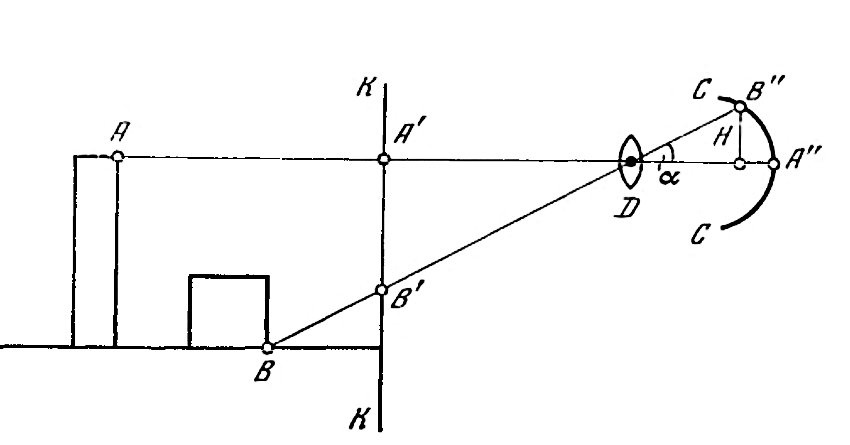
\includegraphics[width=0.8\linewidth]{figures/f1.1.png}
\end{figure}
\figblock{1.1}{Diagram illustrating that central projection onto picture plane $KK$ produces the same retinal image as direct retinal projection, for any retinal surface configuration.}

Consequently, quite independently of the configuration of the retinal surface, the system of
linear perspective ideally serves the purpose of obtaining coinciding retinal images of
external space and of the picture.

If one nevertheless wishes to consider the geometric proximity of the central projection onto
the picture plane $KK$ and onto the spherical surface $CC$, a useful sense of it is given by
comparing the segment $A'B'$ and the arc $A''B''$.  To make this comparison both lines must
be referred to the same scale, which ultimately reduces to comparing the arc-length $A''B''$
subtending visual angle~$\alpha$ and the perpendicular $H$ dropped from $B''$.  Numerically
the ratio of these lengths equals $2\alpha/\sin 2\alpha$ if the eyeball is taken to be
spherical.  This ratio depends strongly on~$\alpha$.  All manuals on the use of linear
perspective in artistic practice state that $\alpha$ should not exceed $15°$.  Another rule
given in drawing manuals specifies that the artist should depict an object from a distance no
less than three times the size of the object; in that case $\alpha < 10°$.  Similar values are
quoted in manuals on the psychology of visual perception as the angle~$\alpha$ corresponding
to sufficiently sharp vision.  This yields a negligibly small departure of arc-length from the
corresponding straight-line segment (of the order of 2--5\%), incomparably smaller than the
transformations brought about by the constancy mechanisms, which can reach hundreds of
per cent.

In view of the fundamental role played by the system of linear perspective here, let us present
the analytical relations belonging to it.  Adopt the following notation (Fig.\,1.2):
$H$---height of the viewpoint; $l_0$---distance from the viewpoint (the artist's eye) to the
picture plane; $b$---distance from the picture plane to the depicted point~$A$, lying in the
subject plane of the picture-space; $B$---distance of point~$A$ from the vertical plane
passing through the principal line of sight (the subject plane is taken to be horizontal);
$y_1$---distance to the image~$A_1$ of point~$A$ on the picture, measured from the base of
the picture plane; $x_1$---distance to the image~$A_1$ of point~$A$ on the picture, measured
from the principal axis of the picture.\footnote{All terms and definitions coincide with those
  given in the textbook by V.\,E.\,Peterson (V.\,E.\,Peterson, \emph{Perspective},
  Moscow, 1970).}

\begin{figure}[H]
    \centering
    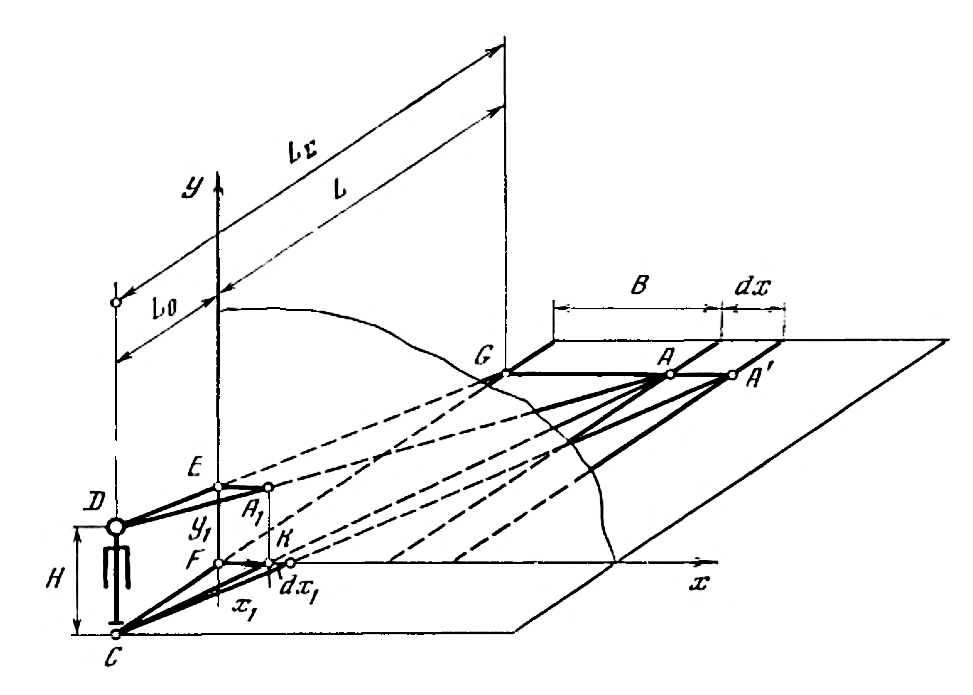
\includegraphics[width=0.9\linewidth]{figures/f1.2.png}
\end{figure}
\figblock{1.2}{Coordinate notation for the linear perspective construction: viewpoint at
  height $H$, picture plane $KK$ at distance $l_0$, depicted point $A$ at depth $b$
  and lateral offset $B$.}

\srcpage{245}

Suppose the problem is to depict a road with parallel edges of width $2B$
($B = \mathrm{const}$), whose axis of symmetry is perpendicular to the picture plane and
passes through the point in the subject plane where the artist stands.

Introduce dimensionless variables
\begin{equation}
  \overline{x} = -\frac{x}{b}, \qquad \overline{y} = \frac{y}{H}, \qquad \overline{l} = \frac{l}{l_0}.
  \tag{1.1}
\end{equation}

It is easy to verify that if the image~$A_1$ of point~$A$ is obtained by central projection
(linear perspective), then from the similarity of triangles $SBO$ and $PEO$ (Fig.\,1.2) there
follows the relation of ordinate~$y_1$ to the distance from point~$A$ to the picture plane:
\begin{equation}
  \overline{y_1} = \frac{l}{l_0 + l} = \frac{\overline{l}}{1+\overline{l}}.
  \tag{1.2}
\end{equation}

The subscript~$1$ here and below signifies that the image~$A_1$ of point~$A$ corresponds to
the system of linear perspective.  The similarity of triangles $SOA$ and $SPK$ allows one to
find the dependence of $x_1$ on~$b$, and with the use of formula~(1.2) to write the relation
between $y_1$ and $x_1$:
\begin{equation}
  \overline{x_1} = \frac{1}{1+\overline{l}},
  \tag{1.3}
\end{equation}
\begin{equation}
  \overline{y_1} = 1 - \overline{x_1}.
  \tag{1.4}
\end{equation}

The last expression says that the curve $y_1 = f(x_1)$ is a straight line; the image of the
road has its true width at the base of the picture plane (at $y_1 = 0$, $x_1 = 1$, i.e.\
$x_1 = B$) and zero width at the horizon line $y_1 = H$, since on that line $y_1 = 1$ and
consequently $x_1 = 0$.  The left edge of the road can be obtained from conditions of
symmetry.

If one takes some elementary segment $dx$ lying in the subject plane and parallel to the
picture plane, then consideration of triangle $CAA'$ shows that the projection of this
segment onto the picture plane will have size $dx_1$, where
\begin{equation}
  d\overline{x_1} = \frac{d\overline{x}}{1+\overline{l}}.
  \tag{1.5}
\end{equation}

Obviously, the size $dx_1$ is exactly the same if the elementary segment $dx$ is translated
parallel to itself to any location in the plane $b = \mathrm{const}$.

\srcpage{246}
